\documentclass[a4paper,12pt]{report}
\usepackage[utf8]{inputenc}
\usepackage[spanish]{babel}
\usepackage{amsmath}
\usepackage{amsfonts}
\usepackage{amssymb}
\usepackage{makeidx}
\usepackage{graphicx}
\usepackage{lmodern}
\usepackage{kpfonts}
\usepackage{apacite}
\usepackage{multirow}
\usepackage{graphicx}
\makeatletter
\renewenvironment{thebibliography}[1]
     {\section*{\bibname}% <-- this line was changed from \chapter* to \section*
      \@mkboth{\MakeUppercase\bibname}{\MakeUppercase\bibname}%
      \list{\@biblabel{\@arabic\c@enumiv}}%
           {\settowidth\labelwidth{\@biblabel{#1}}%
            \leftmargin\labelwidth
            \advance\leftmargin\labelsep
            \@openbib@code
            \usecounter{enumiv}%
            \let\p@enumiv\@empty
            \renewcommand\theenumiv{\@arabic\c@enumiv}}%
      \sloppy
      \clubpenalty4000
      \@clubpenalty \clubpenalty
      \widowpenalty4000%
      \sfcode`\.\@m}
     {\def\@noitemerr
       {\@latex@warning{Empty `thebibliography' environment}}%
      \endlist}
\makeatother
\setlength{\parindent}{0em}
\usepackage{Times}
\usepackage{fancyhdr}
\pagestyle{fancy}
\fancyhead{}
\fancyfoot{}

\rhead{\thepage}
\title{El dengue en Costa Rica: Un análisis espacial}
\author{Pablo Luis Vivas Corrales\\
B57936}
\date{13 de junio, 2020}
\begin{document}
\linespread{1.25}
\maketitle
	
\section*{Introducción}
El dengue es una enfermedad viral que se ha propagado rápidamente en los últimos años. El virus del dengue es transmitido por mosquitos hembras, principalmente de la especie \textit{Aedes aegypti}. Este mosquito también es vector de virus como chikungunya, fiebre amarilla y zika. El dengue está muy extendido en las regiones tropicales y subtropicales \cite{OMS}. La incidencia del dengue ha crecido dramáticamente en todo el mundo en las últimas décadas. La gran mayoría de los casos son leves y autogestionados, y por lo tanto, el número real de casos de dengue no se informa. Muchos casos también se diagnostican erróneamente como otras enfermedades febriles \cite{Waggoner2016}.\\
El virus es altamente transmisible cuando la infestación por el vector es alta, lo que puede producir epidemias de dengue con alta morbilidad y mortalidad, en su forma grave. La infección que produce resulta en un amplio espectro de presentaciones clínicas, que van desde formas asintomáticas, indiferenciadas y leves hasta cuadros graves con compromiso vascular, coagulación y órganos blancos. Puede haber transmisión por la picadura directa del mosquito, vía vertical (madre-hijo,tercer trimestre de embarazo) o vía transfusional \cite{CajaCostarricensedelSeguroSocial2013}.
Los factores de riesgo en la aparición y distribución de la enfermedad se agrupan, principalmente en 2: ambientales y sociales. Sociales como una alta densidad de la población, agua almacenada, ausencia de abastecimiento de agua corriente individual, entre otras. Mientras que ambientales o específicamente geográficos, por localizarse en una zona que favorece la vida del vector que propaga esta enfermedad \cite{factores}, como es el caso de Costa Rica. Solo en el año 2019 la sección de vigilancia del Ministerio de Salud reportó más de 8.000 mil casos de esta enfermedad, siendo el cantón de Sarapiquí de Heredia el cantón más afectado por esta enfermedad (1.816 casos registrados). Por otro lado, al realizar una agregación por provincia, se destacan las provincias de Heredia y de Limón con 1.985 y 1.738 casos respectivamente. \\
Por otro lado se elige realizar técnicas de estadística espacial y de epidemiología pues según \cite{sp} las herramientas de estadística espacial se han utilizado ampliamente en epidemiología al estudio de la distribución de enfermedades. Específicamente, para estudiar el vector \textit{Aedes aegypti}, existe un proyecto costarricense llamado \textit{Mathematical Models for the Development of Prevention/Control Strategies of Aedes Aegypti in Costa Rica} donde los investigadores, en su mayoría matemáticos, crean modelos para fundamentar la toma de decisiones en salud pública con respecto a la propagación del dengue, chikungunya, zika en Costa Rica mediante la identificación y caracterización de métodos de control de Aedes aegypti \cite{ucrea}, sin embargo el enfoque de dicho estudio no se toma en consideración en este artículo pues es un proyecto integral con distintos objetivos. En esta investigación se trabaja de un forma más descriptiva con los siguientes objetivos: (1) identificar la existencia de agrupaciones espaciales en los cantones de Costa Rica (2) determinar indicadores que están asociados con la aparición del dengue y (3) calcular el riesgo que tienen los habitantes de los cantones costarricenses de tener esta enfermedad.\\
Para tomar en cuenta la dependencia espacial,  se realizan modelos jerárquicos Bayesianos, donde para cada cantón se asume que
\begin{align}
y_{i}\sim Poisson(\lambda_{i})  &  & \lambda_{i} = E_{i}\rho_{i}  & & ln(\rho_{i})=\eta_{i}
\end{align}
Donde:
\begin{itemize}
\item $y_{i}$: cantidad de casos observados de dengue en el cantón \textit{i}.
\item $E_{i}$\footnote{Se obtiene multiplicando la tasa de dengue $r_{j} = \frac{\sum y_{ij}}{\sum Pob_{ij}}$ por la cantidad de habitantes de cada cantón $E_{i} = \sum Pob _{ij}* r_{j}$}: cantidad de casos esperados de dengue en el cantón \textit{i}.
\item $\eta_{i} = \beta_{0} + u_{i} + v_{i}$: el componente sistemático del modelo, donde se incluyen las covariables y el efecto espacial ($u_{i}$).
\end{itemize}
Cabe mencionar que varias estructuras se pueden utilizar para la inclusión del efecto especial ($\textbf{u} = {u_{1}, u_{2}, ..., u_{n}}$), sin embargo, en este trabajo utiliza aquella referente a la condicional autoregresiva \cite{sp}. En esta estructura, se consideran \textit{n} áreas, cada una de ellas caracteriszada por un conjunto de vecinos $\mathcal{N}(i)$ y \textit{$u_{i}$} se define como la siguiente variable aleatoria $$u_{i}|u_{-i}\sim Normal \left ( \mu_{i}+\sum_{j=1}^{n}r_{ij}(u_{j}-\mu_{j}), s^{2}_{i}\right )$$
Para más detalles, se puede consultar \cite{sp}
\section*{Métodos}
Los datos utilizados utilizados para realizar el análisis espacial del dengue en Costa Rica provienen de dos fuentes. En primer lugar, de la sección de vigilancia del Ministerio de Salud se obtiene la información de los 8.179 casos de dengue para el 2019 por cantón, al igual que la tasa de dengue (100.000 habitantes). Del censo del 2011 realizado por el Instituto Nacional de Estadística y Censos (INEC) se obtiene las siguiente información: porcentaje de viviendas de tipo tugurio, densidad de la población, porcentaje de viviendas que eliminan los residuos sólidos por camión recolector, porcentaje de viviendas con acueducto. Asímismo, de esta misma institución se extrae la población cantonal para el año 2019.\\
A partir de esos datos se realiza el análisis espacial con el enfoque de estadísticas de áreas y dos enfoques:
\begin{enumerate}
\item[a)] \textit{Enfoque Frecuentista}: Se hace uso de la prueba $\mathcal{I}$ de Moran (al 5\% de significancia) para contrastar la hipótesis de autocorrelación espacial. Asimismo se ajusta un modelo lineal y dos modelos autoregresivos (\textit{SAR \& CAR}) que tratan de describir la tasa de dengue por 100.000 habitantes. Además se ajusta un modelo lineal generalizado quasi-poisson con un término no paramétrico que trata de describir la cantidad de casos de dengue. En estos modelos se emplea el criterio de AIC para seleccionar las variables que tienen más asociación con el fenómeno investigado. Para los cuatro modelos se realiza la prueba de autocorrelación espacial en sus residuos.
\item [b)] \textit{Enfoque Bayesiano}: Se ajustan cuatro modelos jerárquicos con respuesta \textit{Poisson} (mismos modelos que se especificaron en (1)) mediante Aproximación Integrada de Laplace Anidada (\textit{INLA} por sus siglas en inglés) que tratan de describir la cantidad de casos de dengue por cantón. Estos modelos proveniente del área de epidemiología son:  Besag-York-Mollié (BYM) \& Besag, y modificaciones de estos. Cabe señalar que se emplean como distribuciones gamma como previas y los criterios de DIC, WAIC y CPO para selección de modelos.
\end{enumerate}
Para el proccesamiento de los datos se utilizó el software R \cite{R} en su versión 3.6.3 y el IDE RStudio en su versión 1.2.5033. Los paquetes de R utilizados fueron los siguientes: readxl \cite{readxl}, sp \cite{sp}, sf \cite{sf}, tidyverse \cite{tidy}, rgdal \cite{rdal}, RColorBrewer \cite{Rcolor}, spdep \cite{sp}, tmap \cite{tmap}, tmaptools \cite{tmaptools}, spatialreg \cite{sp}, epitools \cite{epitools}, DCluster \cite{dcluster}, plotrix \cite{plotrix}, MASS \cite{MASS},  mgcv \cite{mgcv} \& INLA (cita). Toda la información de este artículo (datos, análisis y resultados) se encuentra disponible en un repositorio de Github que se puede accesar mediante esta dirección: https://github.com/pablo-vivas/Proyecto-Bayesiana.
\section*{Resultados}
Se inicia esta sección con un análisis descriptivo de las variables utilizadas en la investigación. En la figura 1 se presenta la tasa de dengue por 100.000 habitantes.  

\begin{figure}[h!]
\centering
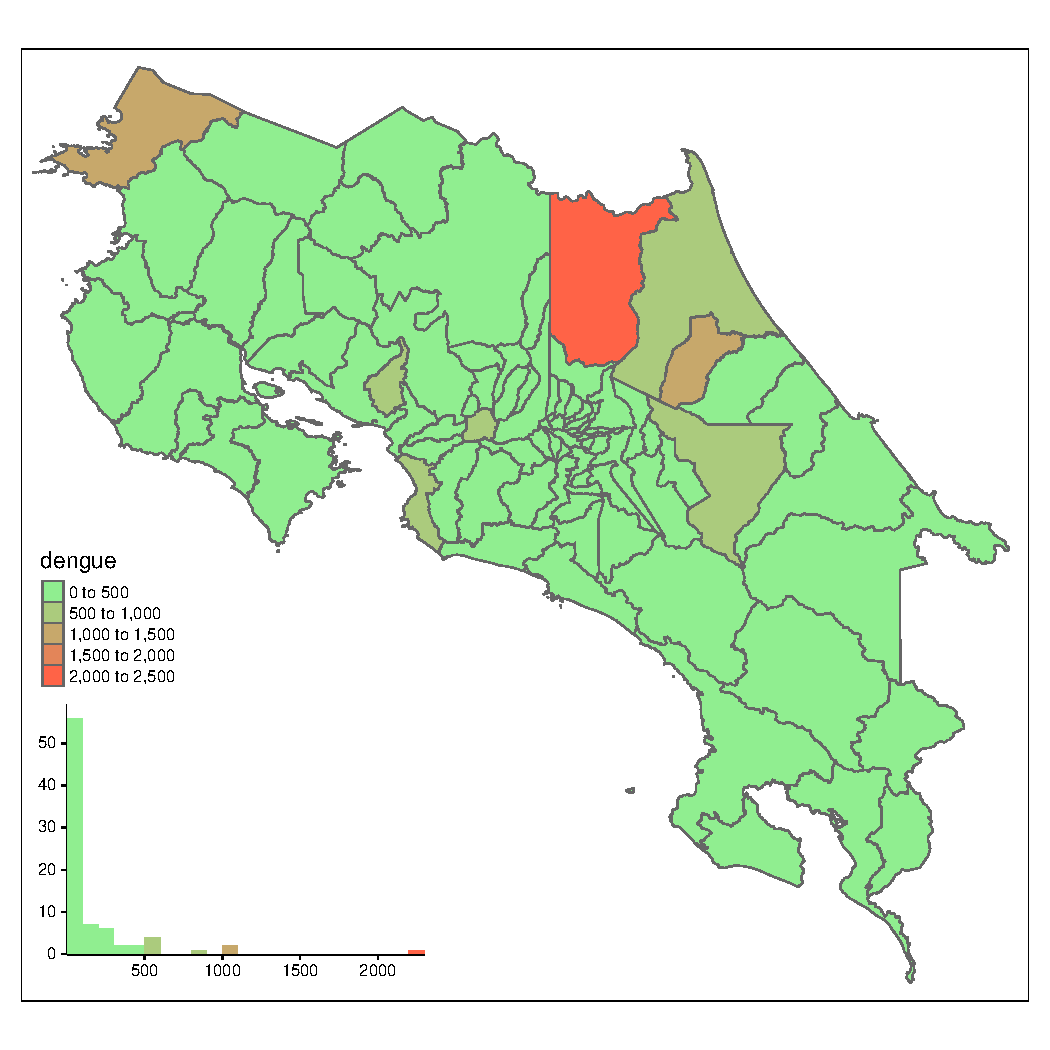
\includegraphics[width=.48\textwidth]{F11.pdf}
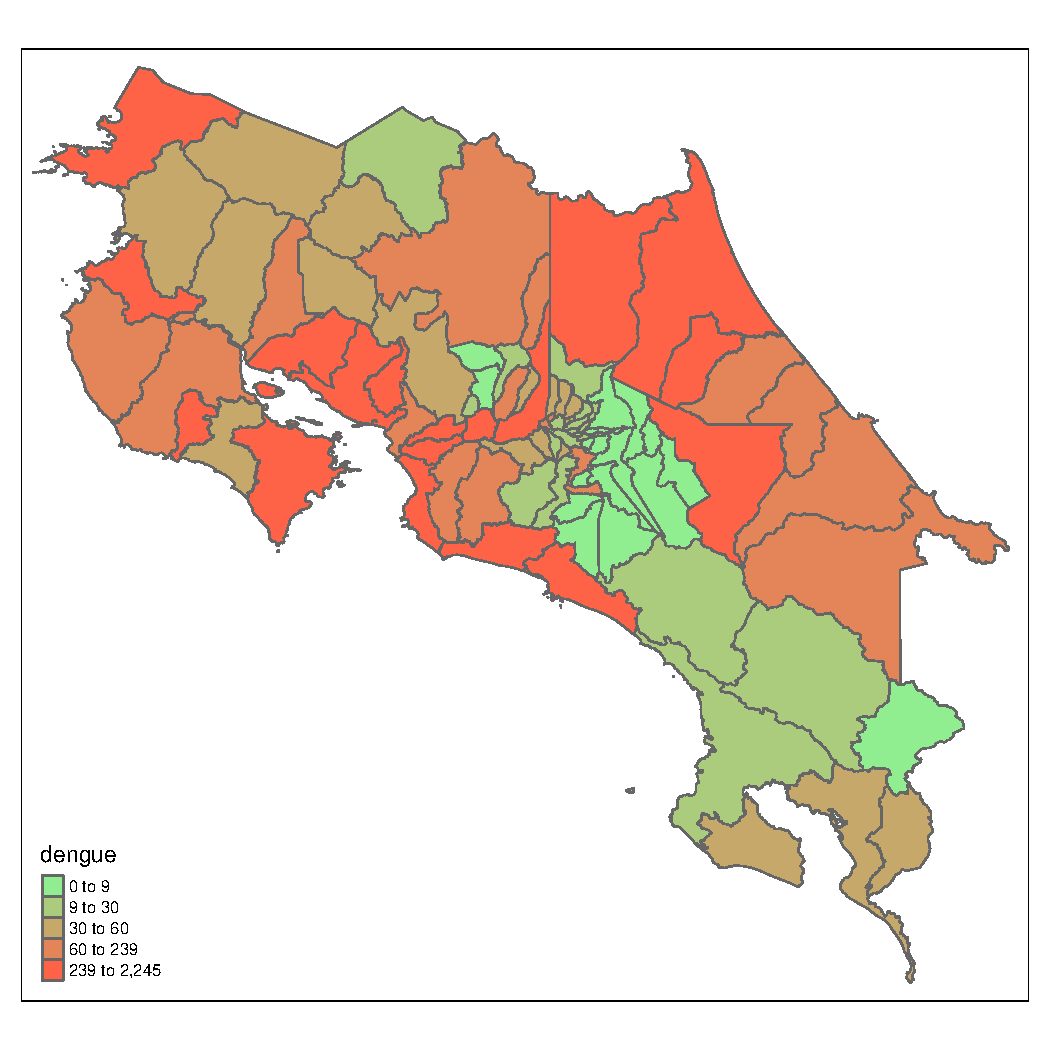
\includegraphics[width=.48\textwidth]{F12.pdf}
\caption{Tasa de dengue (100.000 habitantes) por cantón y tasa de dengue en quintiles por cantón, 2019.}
\end{figure}

Se observa valores altos en los cantones específicos de Sarapiquí, La Cruz, Guácimo y Turrialba, además se incluye un histograma. Con este último gráfico se observa la distribución asimétrica positiva de la tasa de dengue, con un valor extremo muy marcado (Sarapiquí) con una tasa de dengue que sobrepasa los 2.000 por cada 100.000 habitantes, razón por la cual se tiene que mitigar este efecto con un mapa de la tasa de dengue por quintiles, que es el segundo mapa de la primera figura. En ese mapa se presenta una situación similar al primero, tasas elevadas en la región noroeste del país junto con regiones costeras del suroeste. En los anexos se incluyen mapas referidos a los casos de dengue y otra figura que trata de minimizar el efecto del valor extremo mediante el uso de desviaciones estándar.\\
La figura 9 en la sección de anexos presenta la distribución espacial de las covariables utilizadas en el artículo. Dentro de las características más importantes se tiene: porcentajes altos en las zonas de Guanacaste y otras de Alajuela en cuanto a porcentaje de viviendas de tipo tugurio en el 2011, pocos cantones con alta densidad de la población, en la parte central del país  existe una mayor concentración de viviendas que eliminan los residuos sólidos por camión recolector, además las zonas de Guatuso y Upala tienen los porcentajes más bajos en esta variable. Por último en Heredia, Puntarenas y Limón se concentran los porcentajes más bajos de viviendas con acueducto, información relevante es que los cantones de Talamanca y Sarapiquí poseen la mayor cantidad de viviendas sin acueducto.\\ 
Para la definición de la estructura de vecinos y la matriz de pesos, al no tener una referencia clara, se consideran varios métodos. En estructuras de vecinos, se trabajan los métodos de: reina, torre y vecinos más cercanos (Knn) considerando 2 vecinos y 4 vecinos. En la figura 2 se muestra el método de la reina y 4 vecinos más cercanos. Por otra parte, para la matriz de pesos se consideran las estructuras W, B y S, dando como resultado un total de 12 posibles combinaciones de vecinos y matriz de pesos. Se realiza la prueba de $\mathcal{I}$ de moran para cada una de estas combinaciones y los resultados se presentan en la tabla 1. Se concluye que la autocorrelación espacial está presente para cada una de las combinaciones, es decir, no importa cuál estructura de vecino se utilice y cómo se defina la matriz de pesos, los casos y la tasa de dengue en el 2019 posee autocorrelación espacial.
\begin{figure}[hbtp]
\centering
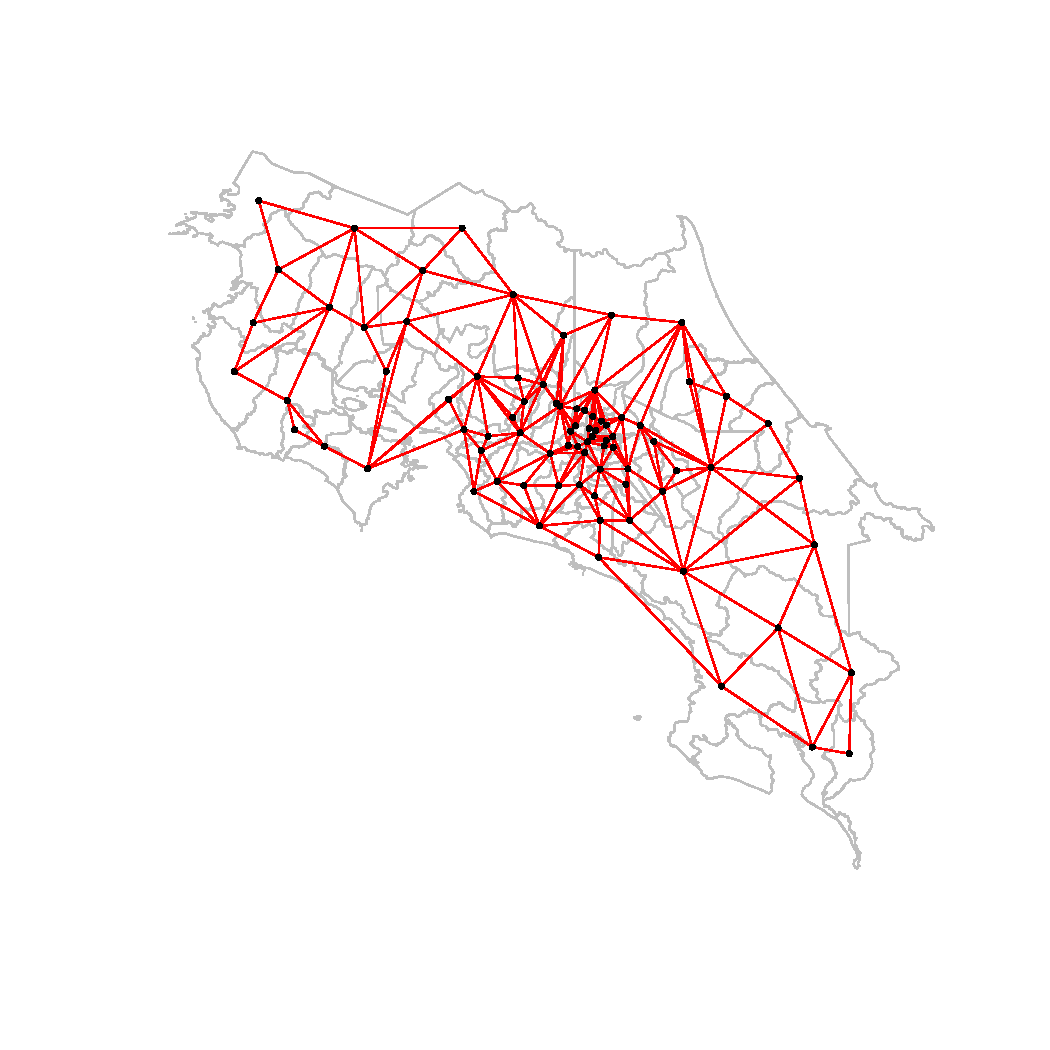
\includegraphics[width=.48\textwidth]{F21.pdf}
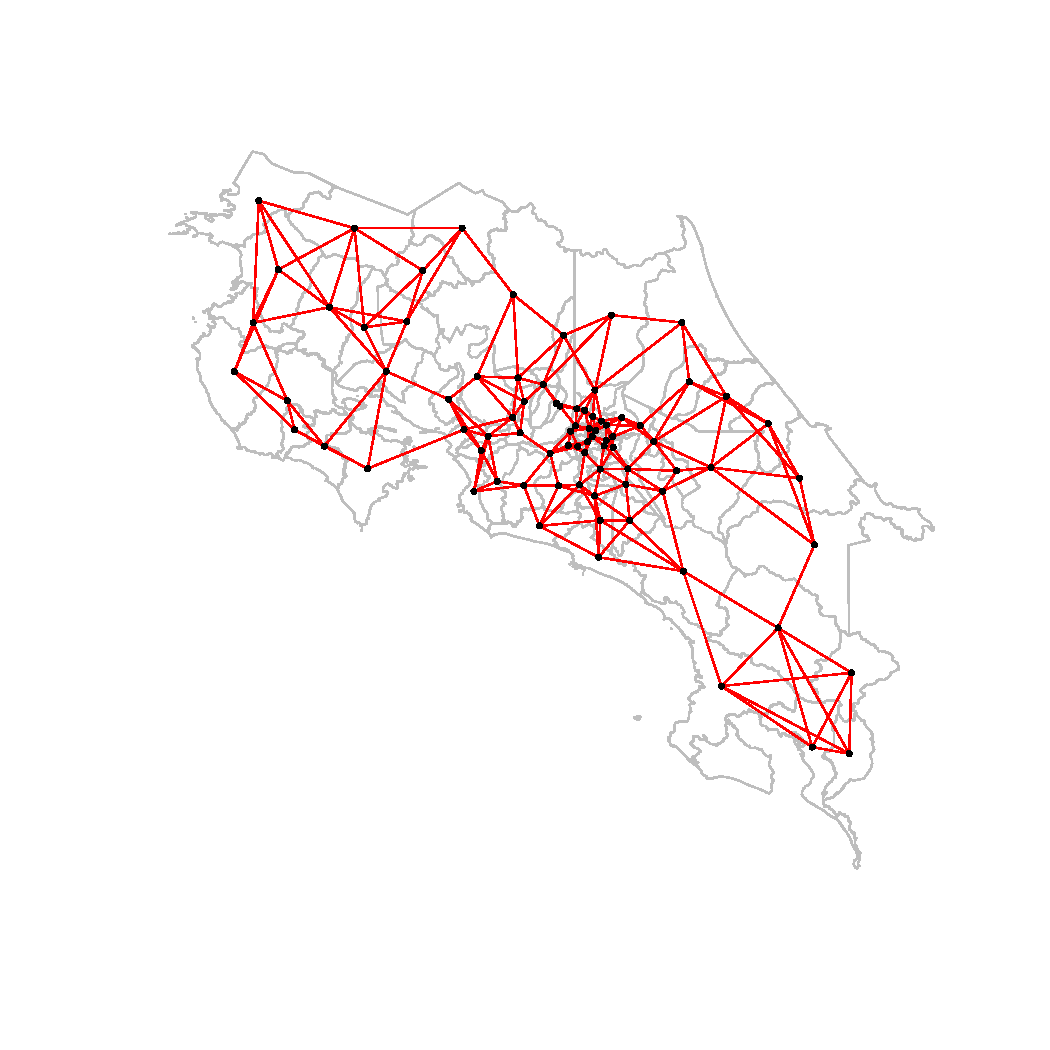
\includegraphics[width=.48\textwidth]{F22.pdf}
\caption{Estructuras de vecinos: Reina y Knn(4)}
\end{figure}

\begin{table}[h]
\centering
\caption{Valores-p para la prueba de autocorrelación espacial según la estrcutura de vecinos y la matriz de pesos}
\begin{tabular}{cccc}
\hline
\multirow{2}{*}{Vecinos} & \multicolumn{3}{l}{Matriz de pesos}\\ \cline{2-4} 
&W&B&S\\ \hline
Reina&0,009&0,007&0,006\\
Torre&0,011&0,008&0,008\\
Knn(2)&0,018&0,018&0,018\\
Knn(4)&0,026&0,026&0,026\\ \hline
\end{tabular}
\end{table}
\newpage

Por otro lado, se ajusta un modelo lineal (con tranformación raíz cuadrada en la variable respuesta) y dos modelos autoregresivos (\textit{SAR \& CAR}) que tratan de describir la tasa de dengue por 100.000 habitantes y un modelo lineal generalizado quasi-poisson con un término no paramétrico que trata de describir la cantidad de casos de dengue. Para cada uno de estos modelos se emplea el criterio AIC para determinar las covariables que resultan importantes para describir el fenómeno en cuestión. En los cuatro modelos las variables porcentaje de viviendas que eliminan los residuos sólidos por camión recolector y porcentaje de viviendas con acueducto resultan ser significativas al 5\% y minimizan el AIC en cada escenario. Este es un resultado esperado, pues se evidenció en el análsis descriptivo que estas variables presentan comportamiento similar a la tasa de dengue y a los casos de dengue en el 2019.\\
Los residuales de estos modelos se presentan en la figura 3, donde resalta que los dos modelos autoregresivos tienen problemas con el cantón de Sarapiquí y aledaños, mientras que los residuales de los  otros dos modelos son pequeños en comparación con los residuales de los modelos autoregresivos. Cabe destacar que al realizar la prueba de autocorrelación espacial para los residuales de cada uno de los cuatro modelos, solo los modelos autorregresivos no tienen rastro de componente de autocorrelación. Por otro lado, el modelo quasi-poisson con término no paramétrico de suavizamiento, explica aproximadamente el 88\% de la deviancia y posee un $R^{2}$ ajustado de 93\%, lo que quiere decir que un buen modelo para estos datos, sin embargo se sospecha un sobreajuste del término no paramétrico.

\begin{figure}[hbtp]
\centering
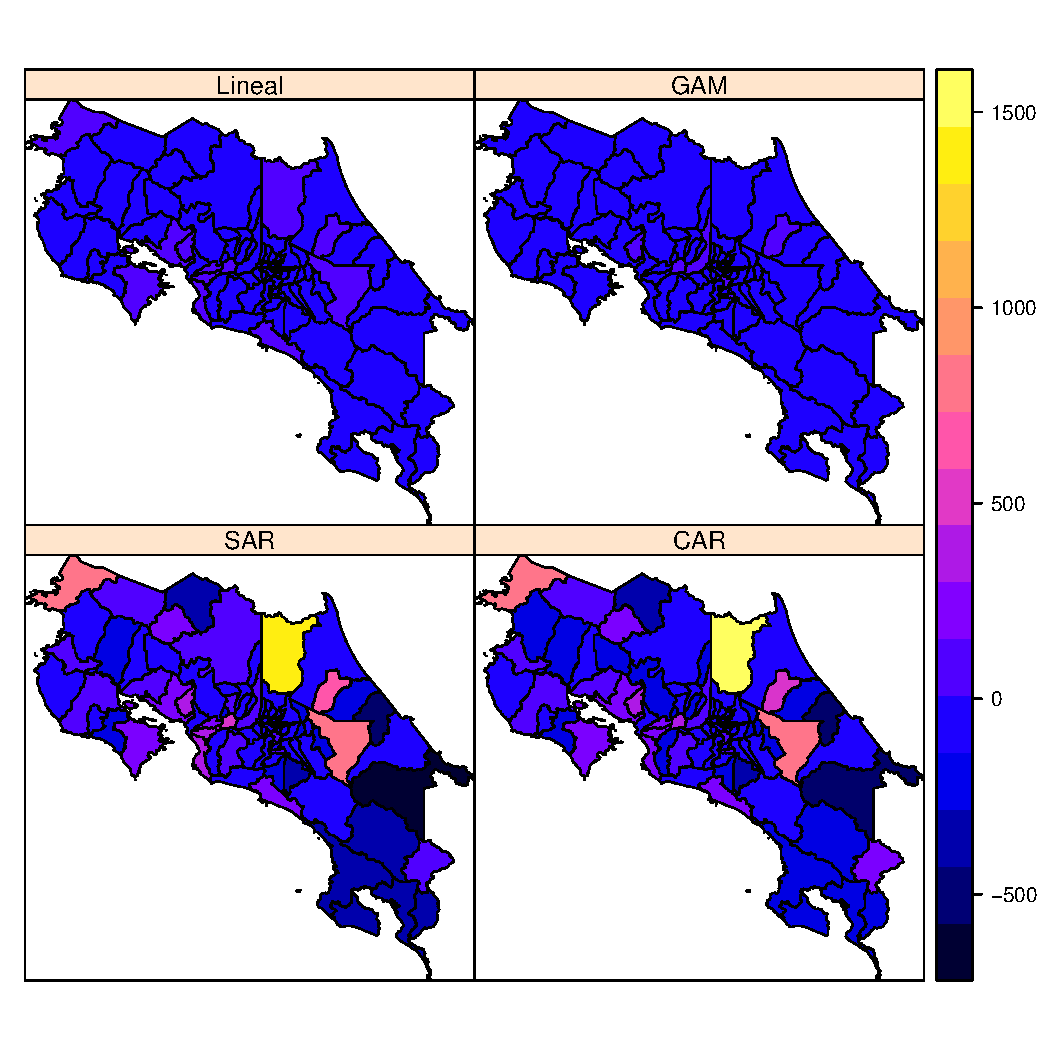
\includegraphics[scale=0.45]{F4.pdf}
\caption{Residuales de los cuatro modelos ajustados}
\end{figure}

\newpage
Se prosigue con un análisis epidemiológico con el cálculo del riesgo relativo, o SMR (Standardised Mortality Ratio) \cite{sp} y su respectiva graficación en la figura 5, que además se completa con la figura 6, donde se muestran los intervalos de confianza del 95\% para el riesgo relativo de cada cantón. Aquí se destacan 8 cantones cuyo riesgo relativo resulta significativo: Sarapiquí, Guacimo, La Cruz, Turrialba, Atenas, Montes de Oro, Garabito y Pococí, es decir, una persona de Sarapiquí es hasta 22 veces más probable de enfermarse de dengue y una persona de Guácimo hasta 13 veces más probable.
\begin{figure}[hbtp]
\centering
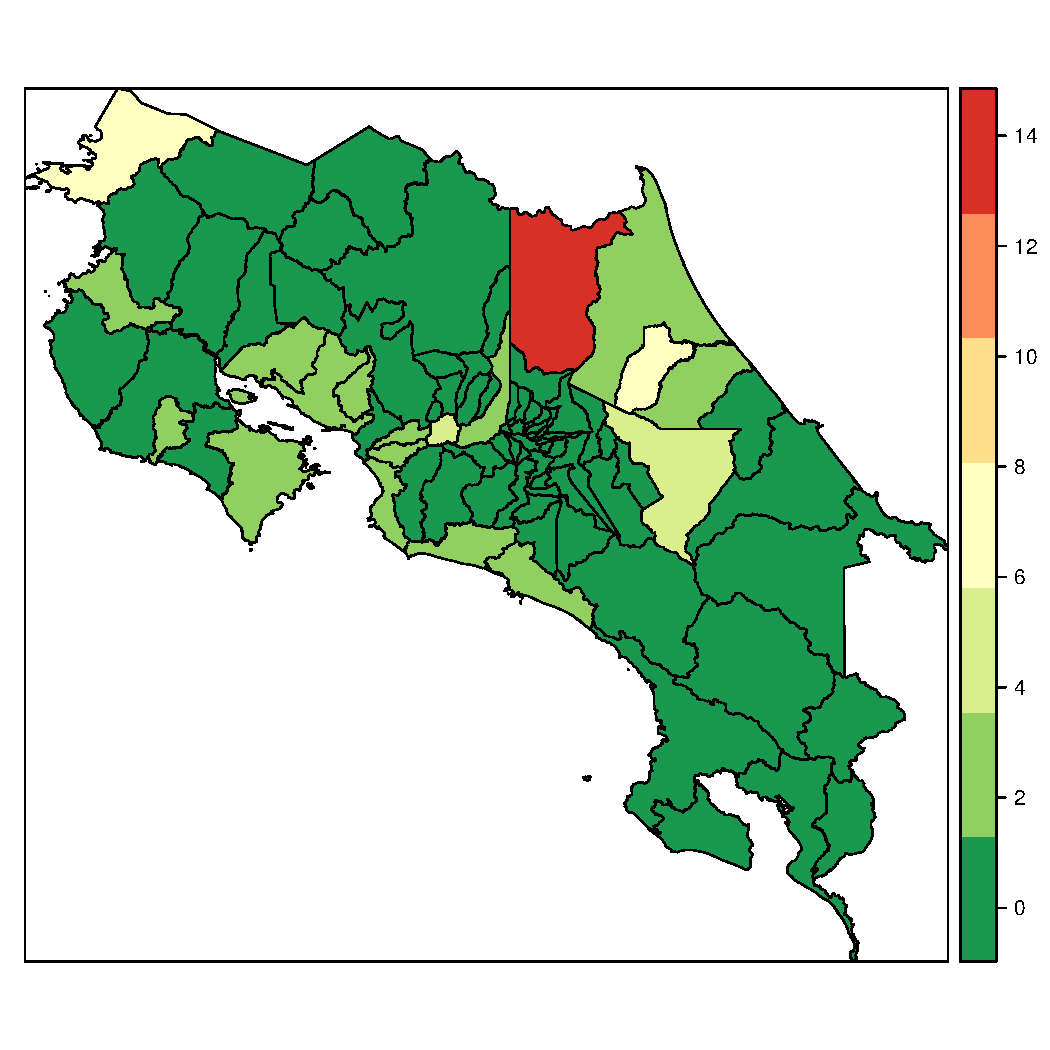
\includegraphics[scale=0.48]{F5.pdf}
\caption{Riesgo relativo}
\end{figure}

\begin{figure}[t]
\centering
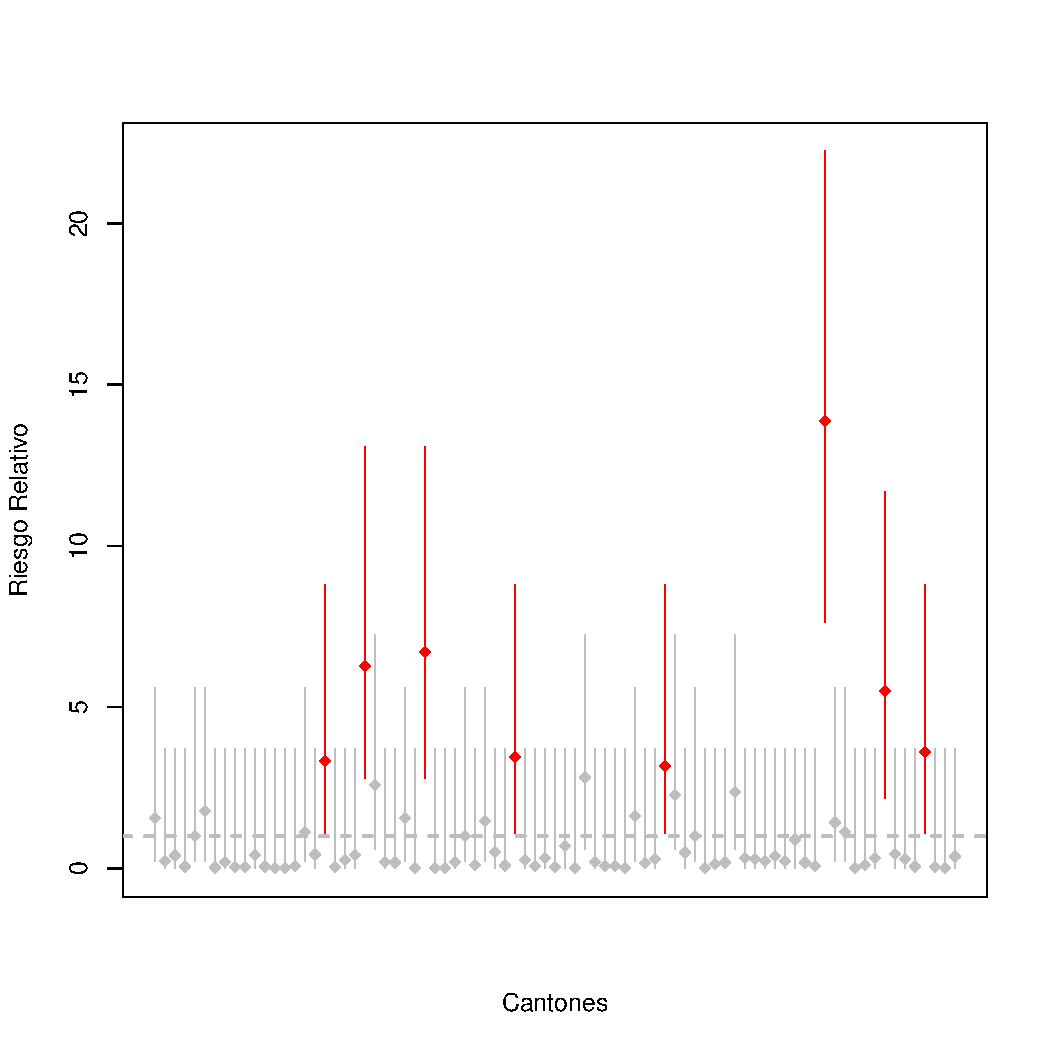
\includegraphics[scale=0.46]{F6.pdf}
\caption{Intervalos de confianza del 95\% para el riesgo relativo de dengue, por cantón. Los intervalos en rojo corresponden a los cantones de: Garabito, Guácimo, La Cruz, Montes De Oro, Pococí, Sarapiquí, Turrialba y Atenas}
\end{figure}

Cambiando al enfoque Bayesiano, se ajustan cuatro modelos jerárquicos con respuesta de \textit{Poisson} para describir la cantidad de casos de dengue por cantón. Los modelos considerados en esta investigación son: Besag, Besagporper (esto porque el modelo Besag utiliza distribuciones impropias), BYM y por último IID (independiente e idénticamente distribuido). En cada uno de estos modelos se realiza primero una selección de variables mediante el criterio del DIC y se llega a la misma estructura que en la parte frecuentista, es decir, se eligen como candidatos los modelos con las siguientes covariables: porcentaje de viviendas que eliminan los residuos sólidos por camión recolector y porcentaje de viviendas con acueducto. Cabe resaltar que los cuatro modelos alcanzan la convergencia muy fácilmente, esto se debe al uso de un modelo conocido y al uso del algoritmo \textit{INLA} que es una buena alternativa a los métodos clásicos de MCMC.\\
 Por otro lado, se comparan estos cuatro modelos mediante los siguientes estadísticos: DIC, WAIC (\textit{Widely Applicable Information Criterion}), y CPO (\textit{Conditional Predictive Ordinate}) y los resultados se muestran en la tabla 2. Se puede observar que los cuatro modelos funcionan muy similar y tienen resultados parecidos para cada uno de los criterios de comparación, existen pequeñas diferencias en el DIC y en el WAIC, mienras que en el estadístico de CPO se presentan las diferencias más grandes. A la luz de estos resultados se puede utilizar cualquiera de estos cuatro modelos para análisis posteriores.

\begin{table}[hbtp]
\centering
\caption{Estadísticos para los modelos jerárquicos}
\begin{tabular}{cccc}
\hline
\multirow{2}{*}{Modelo} & \multicolumn{3}{l}{Estadístico}\\ \cline{2-4} 
&DIC&WAIC&CPO\\ \hline
Besag&541,23&525,18&-478,96\\
Besagproper&541,48&525,45&-415,69\\
BYM&547,01&533,98&-409,47\\
IID&546,55&533,07&-425,09\\ \hline
\end{tabular}
\end{table}

\begin{figure}[t]
\centering
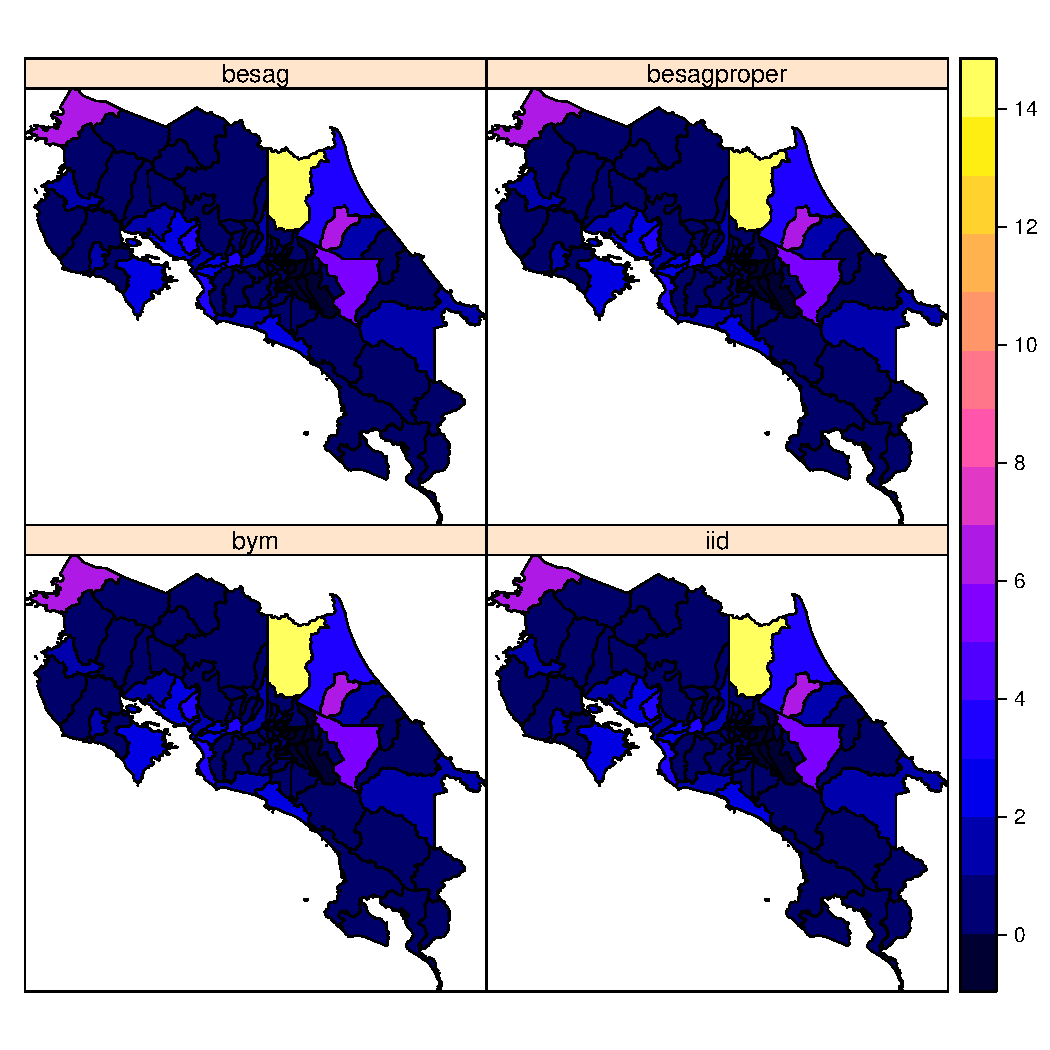
\includegraphics[scale=0.45]{FF2.pdf}
\caption{Riesgo relativo de dengue, para los cuatro modelos jerárquicos.}
\end{figure}

\begin{table}[h!]
\centering
\caption{Estimaciones de los coeficientes para los cuatro modelos jerárquicos}
\begin{tabular}{llllll}
\hline
                  Coeficiente&Promedio &Desv.Estándar &$P_{2,5}$ &  $P_{50}$& $P_{97,5}$ \\ \hline
\multirow{3}{*}{$\hat{\beta}_{0}$}& 4,564& 2,139&  0,338&4,570&8,754     \\
                  & 4,016& 2,178&  -0,304&4,026&8,276 \\
                  & 4,585& 2,070&  0,0500&4,587&8,656 \\
                  & 4,571& 2,144&  0,0342&4,573&8,784\\ \hline
\multirow{3}{*}{$\hat{\beta}_{1}$}& 0,025& 0,013&  0,000&0,025&0,050     \\
                  & 0,021& 0,013&  -0,005&0,021&0,047 \\
                  & 0,008& 0,012&  0,001&0,008&0,030 \\
                 & 0,008& 0,013&  0,001&0,008&0,031\\ \hline
\multirow{3}{*}{$\hat{\beta}_{2}$}& -0,085& 0,028&  -0,140&-0,085&-0,031     \\
                  & -0,076& 0,028&  -0,131&-0,076&-0,077   \\
                  & -0,070& 0,029&  -0,127&-0,070&-0,070   \\
                 & -0,070& 0,030&  -0,129&-0,070&-0,031 \\ \hline
\end{tabular}
\end{table}

 Asimismo, se calculan los riegos relativos para los cantones de Costa Rica, en cada uno de estos modelos y algunos estadísticos referentes a los coeficientes estimados. Los resultados se muestran en la figura 6 y en la tabla 3, respectivamente.\\
Una vez más, los resultado apuntan a que los cuatro modelos trabajan de forma similar. Además las estimaciones de los parámetros es buena y se captura la información espacial. Se puede notar como los modelos replican de buena forma el riego relativo presentado en la figura 4. Además, se calculan los intervalos de credibilidad del 95\% para esos riesgos relativos. El resultado se presenta en la figura 7.

\begin{figure}[hbtp]
\centering
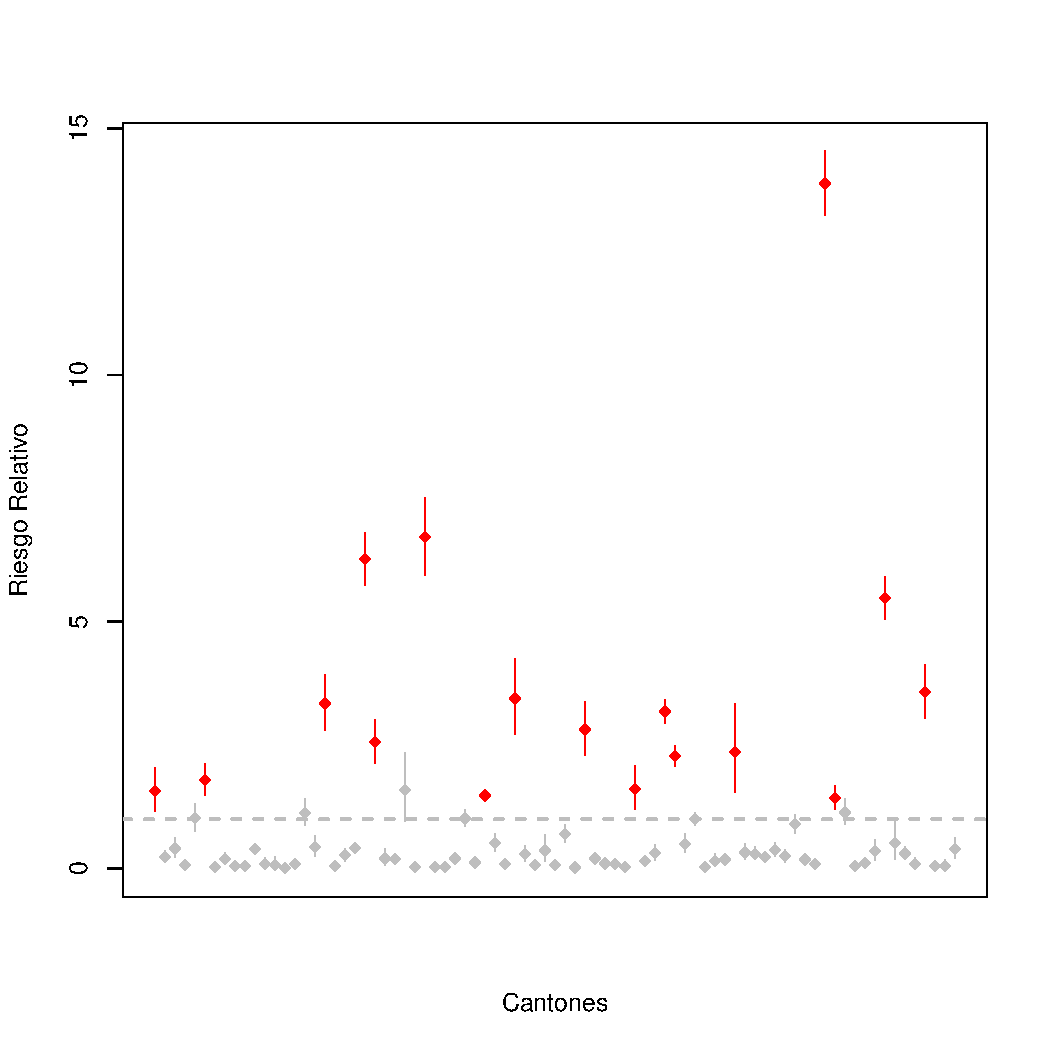
\includegraphics[scale=0.55]{FF1.pdf}
\caption{Intervalos de credibilidad del 95\% para el riesgo relativo de dengue, por cantón. Los intervalos en rojo corresponden a los cantones de: Abangares, Carrillo, Garabito, Guácimo, Aguirre, La Cruz, Alajuela, Montes De Oro, Orotina, Parrita, Pococí, Puntarenas, San Mateo, Sarapiquí, Siquirres, Turrialba y Atenas}
\end{figure}
De estos intervalos de credibilidad se puede destacar que son mucho más angostos que los intervalos calculados con el enfoque frecuentista, esto permite que más cantones tengan un límite inferior mayor a 1, con lo que su riesgo de contraer dengue ya es relevante para este estudio. Además para los cantones que ya tenían esta característica  en el enfoque frecuentista, también lo será en el enfoque bayesiano. Se puede tomar de ejemplo el cantón de Sarapiquí, cuyo intervalo de confianza era $[7,18; 22,41]$ aproximadamente y su intervalo de credibilidad es de $[13,25; 14,53]$ aproximadamente, siendo más preciso este último.
\newpage


\section*{Discusión}
Por medio del análisis realizado se concluye que la ditribución de los casos de dengue y la tasa de dengue por 100.000 habitantes en el territorio de Costa Rica no es aleatoria, sino que existen patrones espaciales que se deben tomar en consideración, es decir, se evidenció la existencia de autocorrelación espacial. Además esta autocorrelación no depende de la estructura de vecinos ni de la selección de matriz de pesos que se elija, debido a que son muy evidenctes las agrupaciones espaciales que existen. También se determinó que la tasa de dengue por 100.000 habitantes puede ser explicada de gran forma mediante un modelo generalizado quasi-poisson con un término no paramétrico de suavizamiento (en el enfoque frecuentista) y que las variables están asociadas a este fenómeno son el porcentaje de viviendas que eliminan los residuos sólidos por camión recolector y el porcentaje de viviendas con acueducto.. Además que los habitantes de los cantones de Sarapiquí, Guacimo, La Cruz, Turrialba, Atanas, Montes de Oro, Garabito y Pococí tienen un riesgo mayor de contraer dengue y que se puede dedicar campañas de prevención en los cantones de San Carlos, Limón y Talamanca, entre otros. \\
Por otro lado, el análisis Bayesiano demuestra que esos intervalos de confianza son muy amplios y al usar un modelo jerárquico con respuesta \textit{Poissson}, los intervalos de credibilidad pueden ser muy estrechos, por ejemplo, en Sarapiquí el riego relativo pasa de un intervalo de confianza de $[7,18; 22,41]$ (aproximadamente) a un intervalo de credibilidad es de $[13,25; 14,53]$ (aproximadamente). Asimismo se evidenció la compatibilidad de varios modelos con las observaciones obtenidas. Los modelos epidemiológicos utilizados (Besag, Besagproper, BYM e IID) funcionan de una forma muy similar en este contexto, y no hubo un claro ganador al comparar estadísticos para la selección de modelos (DIC, WAIC) ni en la validación cruzada (CPO). También se analizó la distribución posterior de los coeficientes del modelo ($\beta_0,\beta_1,\beta_2$) y se encontró similitudes en estos cuatros modelos. La combinación de enfoques frecuentistas y bayesianos en el análisis espacial de áreas, enriquese la comprensión del fenómeno en cuestión y en este trabajo empleó un subconjunto de herramientas disponibles para la modelación espacial.Es menester resaltar la carencia de investigaciones similares a esta, para el estudio de enfermedades virales como el dengue en las regiones tropicales. Esto se debe en parte a la disponibilidad computacional de las técnicas de MCMC por medio de \textit{INLA} .
\newpage
%%Bibliografía
\bibliographystyle{apacite}
\bibliography{Referencias}

\newpage
\section*{Anexos}

\begin{figure}[hbtp]
\centering
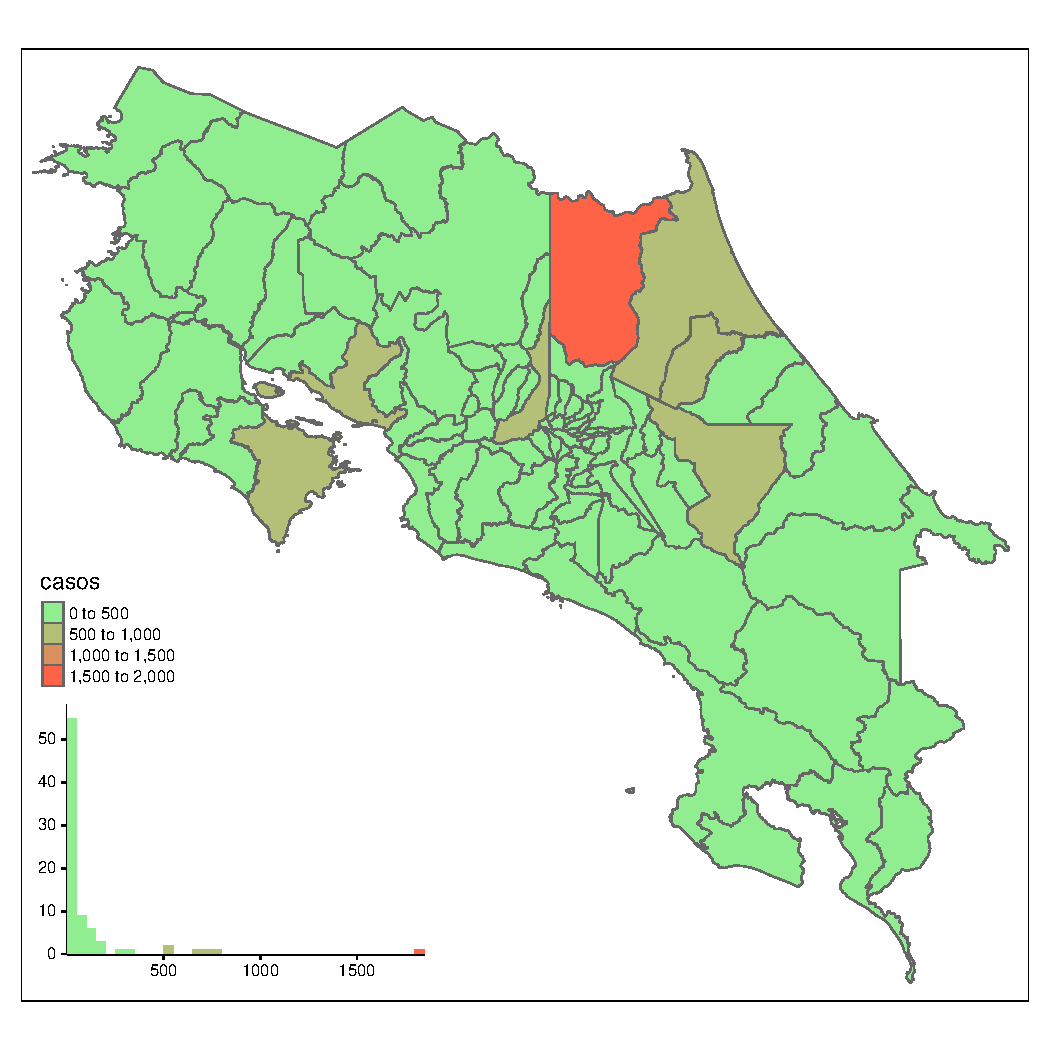
\includegraphics[width=.48\textwidth]{FA1.pdf}
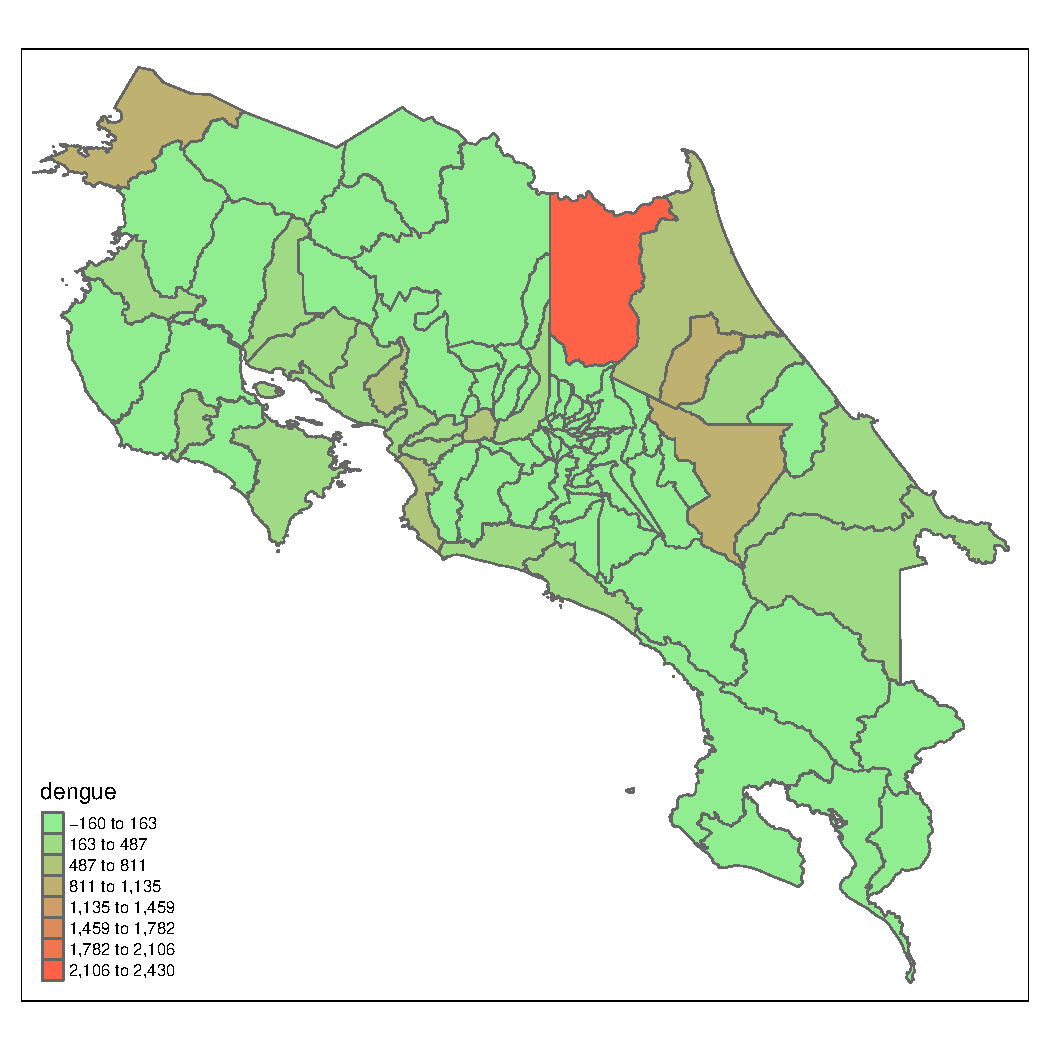
\includegraphics[width=.48\textwidth]{FA2.pdf}
\caption{Casos de dengue por cantón y desviación estándar de la tasa de dengue por 100.000 habitantes, 2019.}
\end{figure}
\newpage
\begin{figure}[hbtp]
\centering
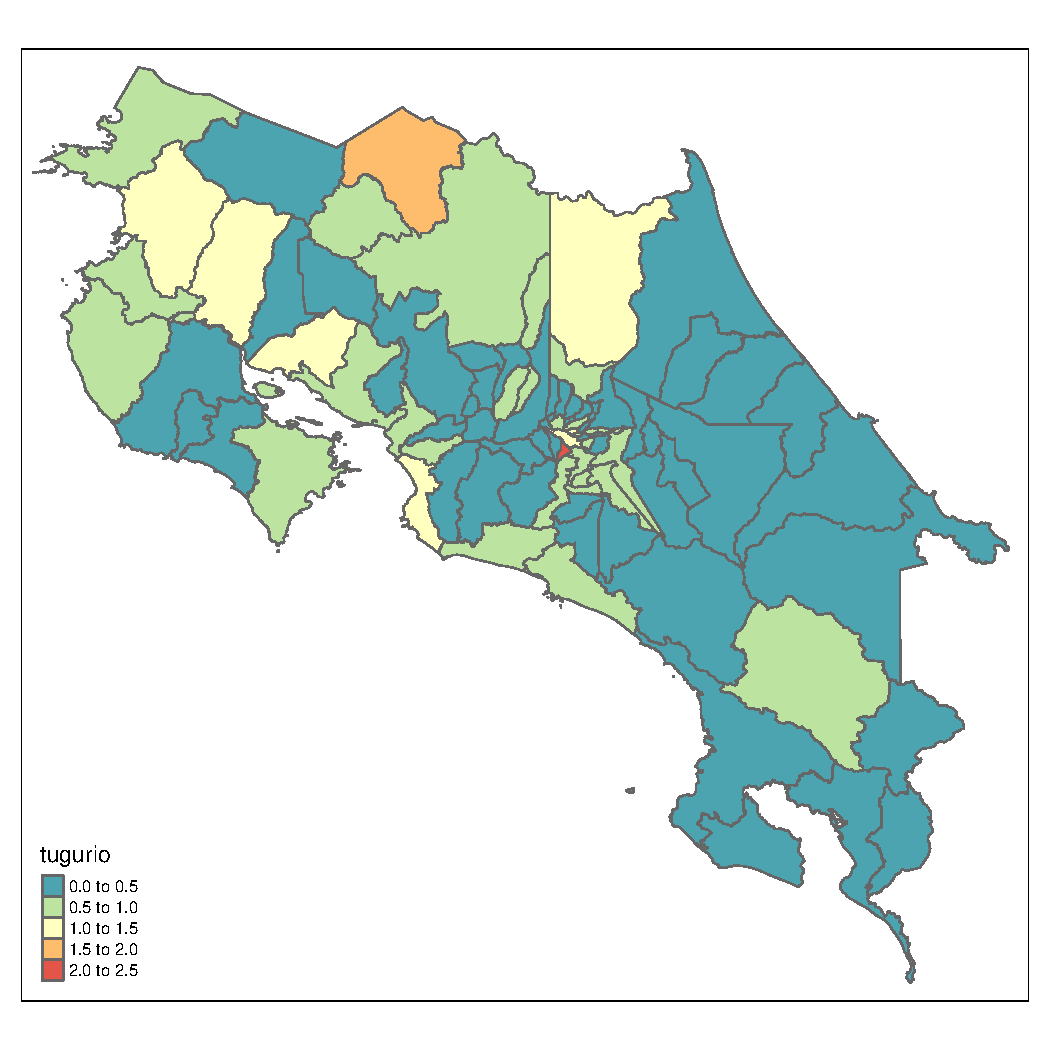
\includegraphics[width=.48\textwidth]{FA3.pdf}
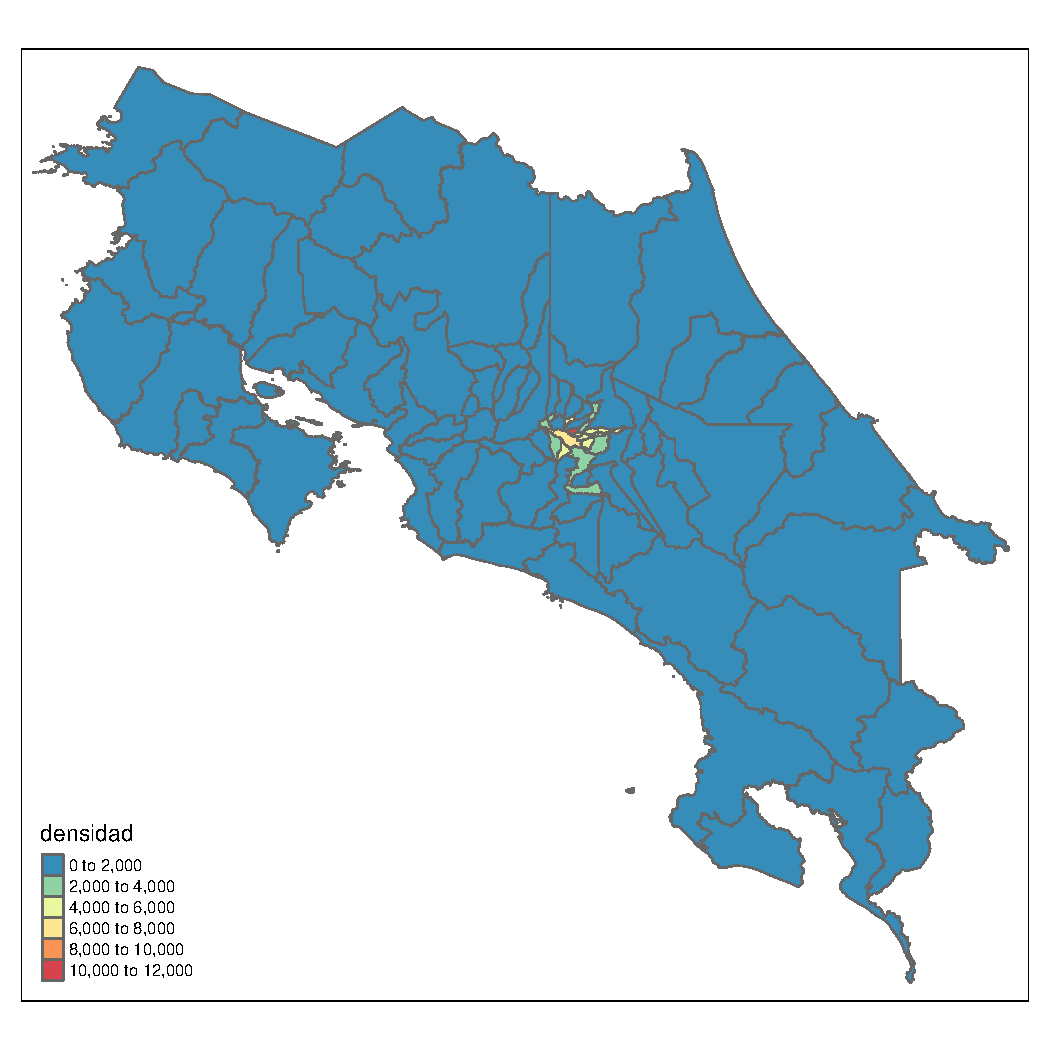
\includegraphics[width=.48\textwidth]{FA4.pdf}
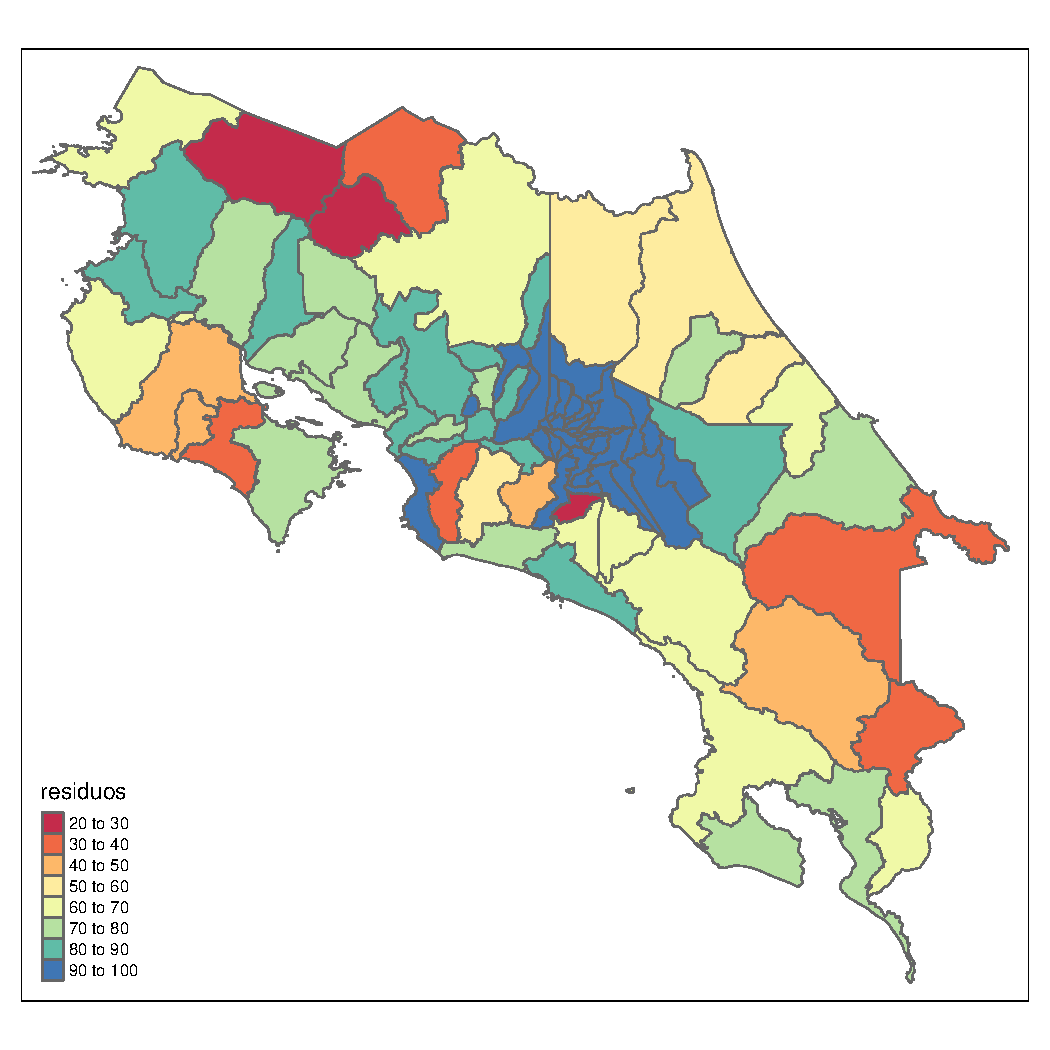
\includegraphics[width=.48\textwidth]{FA5.pdf}
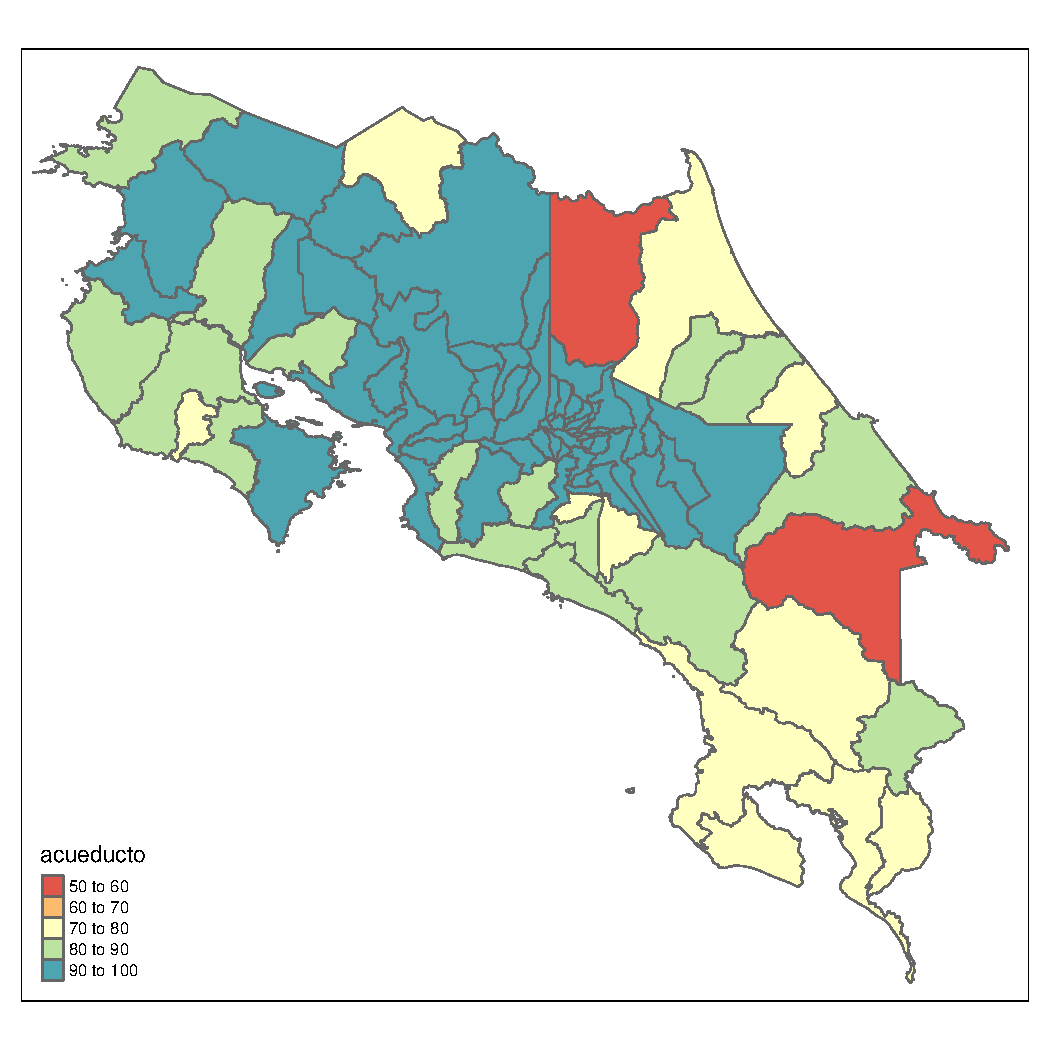
\includegraphics[width=.48\textwidth]{FA6.pdf}
\caption{Porcentaje de viviendas de tipo tugurio, densidad de la población, porcentaje de viviendas que eliminan los residuos sólidos por camión recolector, porcentaje de viviendas con acueducto}
\end{figure}
\newpage
\begin{figure}[hbtp]
\centering
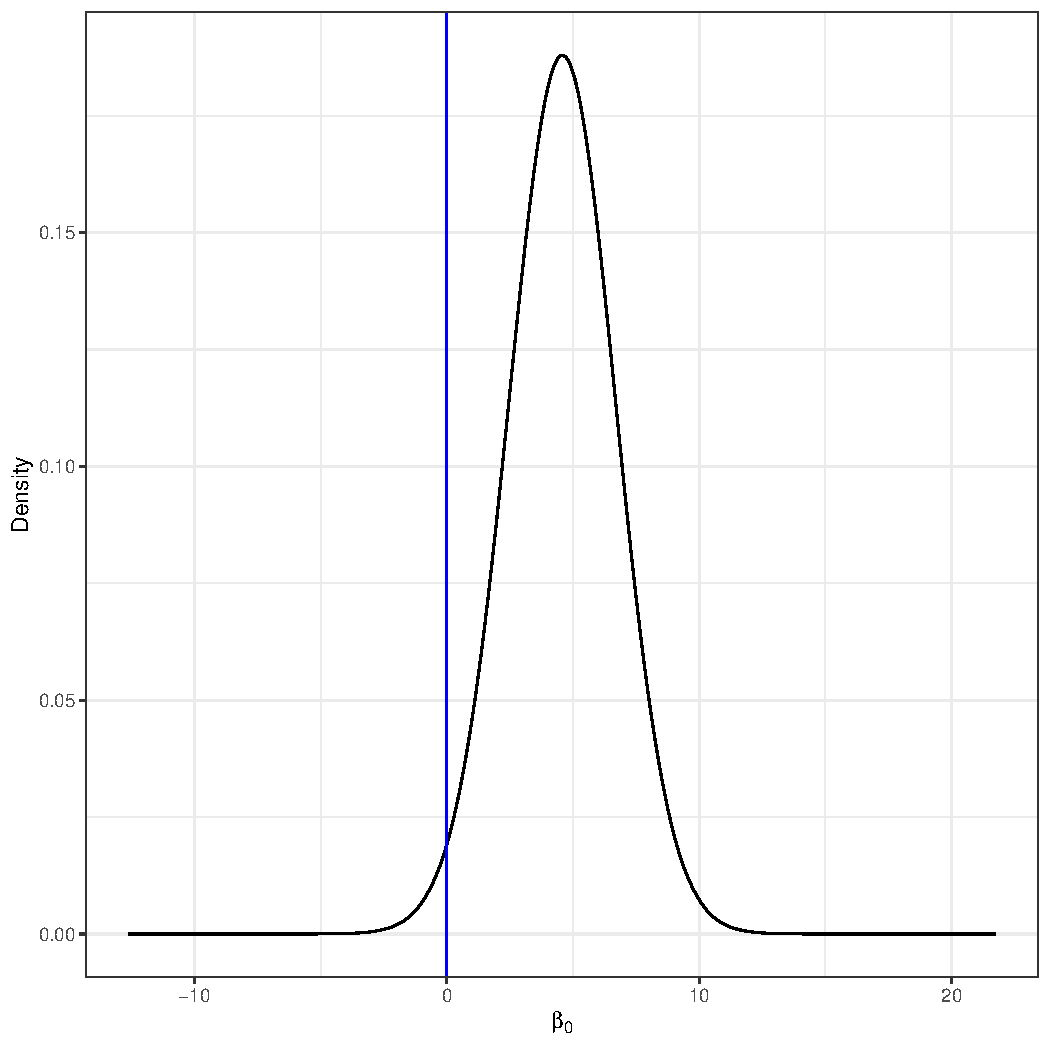
\includegraphics[width=.48\textwidth]{FF31.pdf}
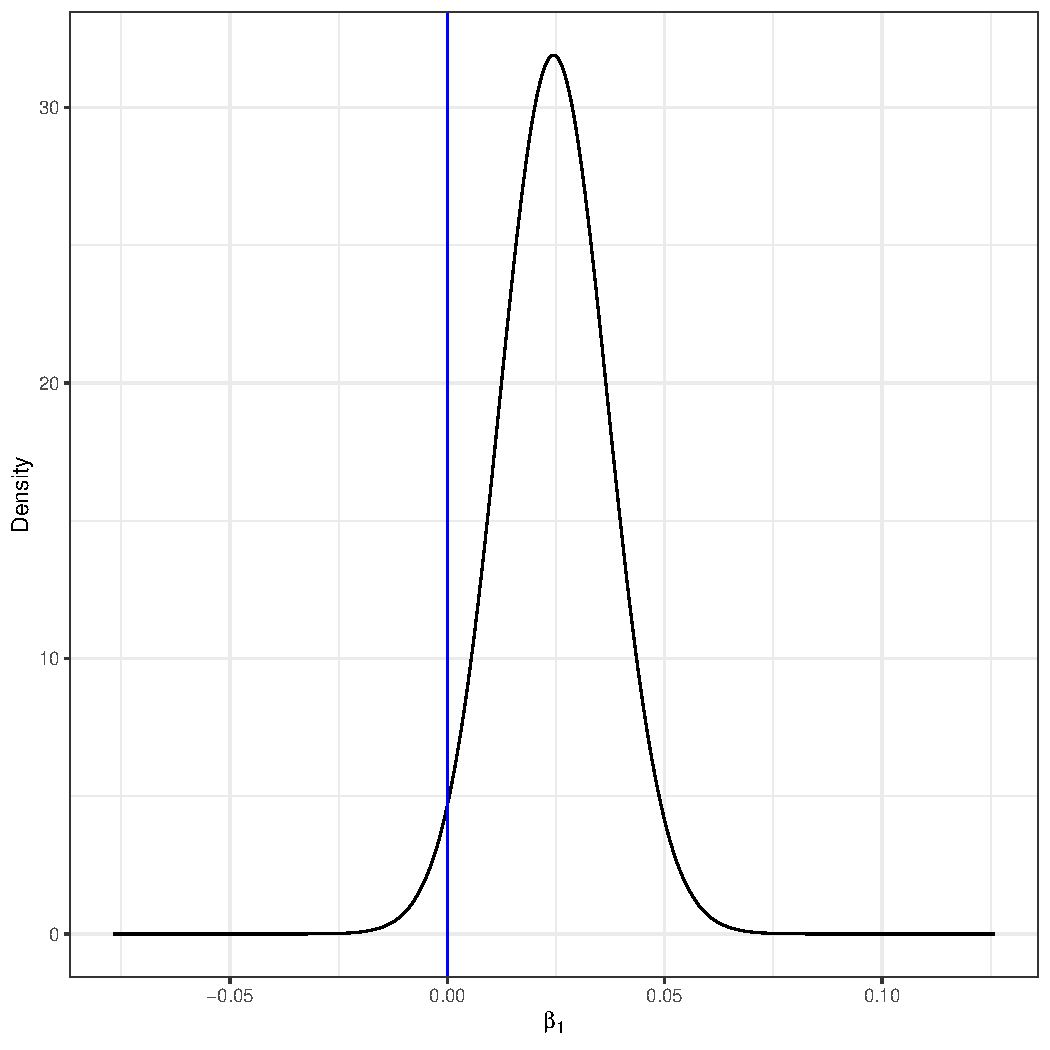
\includegraphics[width=.48\textwidth]{FF32.pdf}
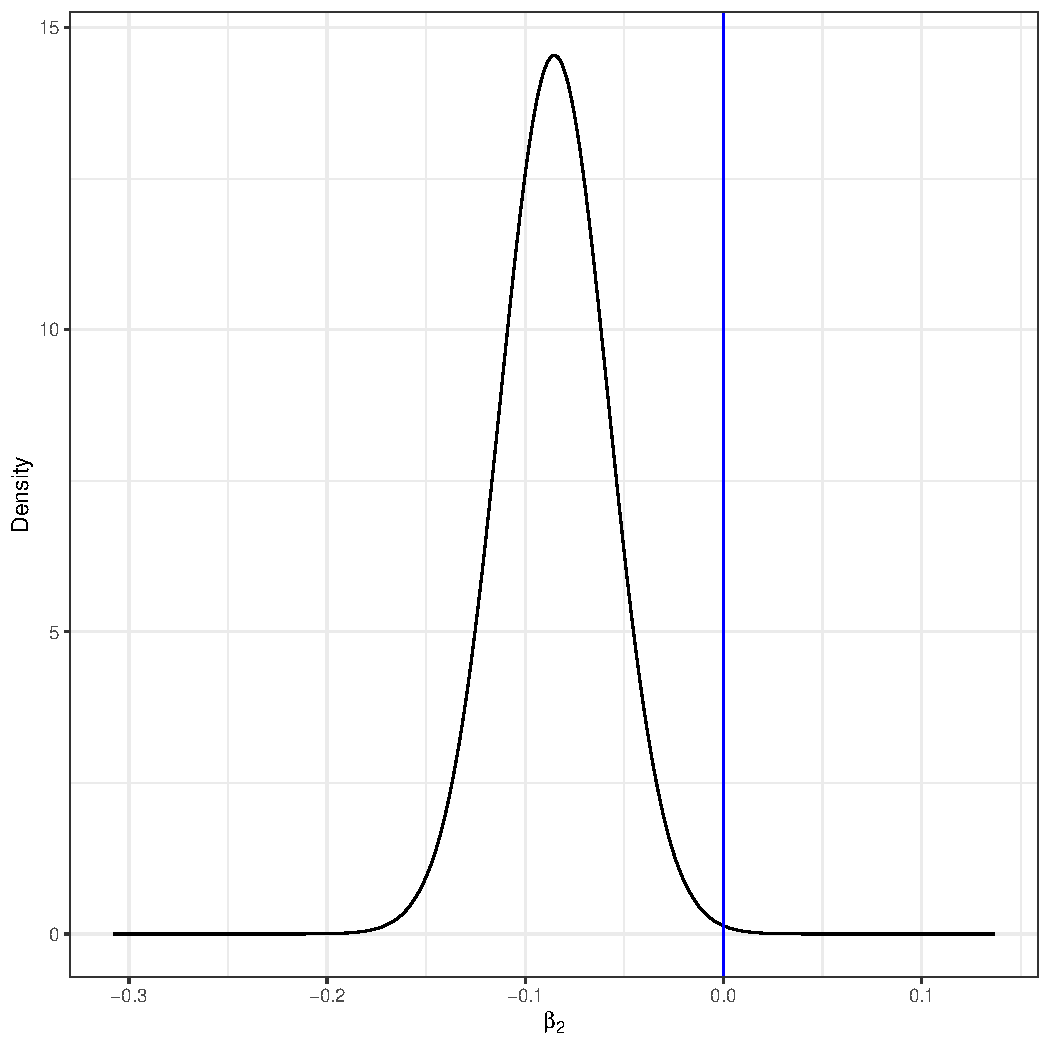
\includegraphics[width=.48\textwidth]{FF33.pdf}
\caption{Distribución posterior de los parámetros}
\end{figure}
\newpage

\subsection*{Código empleado}
\begin{verbatim}
##Análisis

#Librerías
library(readxl)
library(sp)
library(sf)
library(tidyverse)
library(rgdal)
library(RColorBrewer)
library(spdep)
library(tmap)
library(tmaptools)
library(spatialreg)
library(epitools)
library(DCluster)
library(plotrix)
library(MASS)
library(mgcv)
library(INLA)

indicadores <- read_excel("Datos/Datos Cantonales.xlsx")
cantones_sp <- read_sf(dsn="Datos",layer = "Cantones")

#Merge
datos_sf <- merge(cantones_sp,indicadores)
datos_sf <- datos_sf[,-c(1:4)]
rm(cantones_sp,indicadores)

#Quitar la Isla del Coco
new_bb = c(286803.0, 889158.2, 658864.2,1241118.1)
names(new_bb) = c("xmin", "ymin", "xmax", "ymax")
attr(new_bb, "class") = "bbox"
attr(st_geometry(datos_sf), "bbox") <- new_bb
rm(new_bb)

datos_sf2 <- datos_sf


# Primer ploteo -----------------------------------------------------------


#Estadísticas descriptivas
#pdf("Trabajo Escrito/F11.#pdf")

tm_shape(datos_sf) +
  tm_polygons("dengue", palette=c("lightgreen","tomato"), legend.hist=TRUE)

#dev.off()

#pdf("Trabajo Escrito/F12.#pdf")

tm_shape(datos_sf) +
  tm_polygons("dengue", palette=c("lightgreen","tomato"),style="quantile")

#dev.off()

#pdf("Trabajo Escrito/FA1.#pdf")

tm_shape(datos_sf) +
  tm_polygons("casos", palette=c("lightgreen","tomato"), legend.hist=TRUE)

#dev.off()

#pdf("Trabajo Escrito/FA2.#pdf")

tm_shape(datos_sf) +
  tm_fill("dengue",style="sd",palette=c("lightgreen","tomato")) +
  tm_borders()

#dev.off()

#pdf("Trabajo Escrito/FA3.#pdf")

tm_shape(datos_sf) +
  tm_polygons("tugurio",n=6, palette="-Spectral")

#dev.off()

#pdf("Trabajo Escrito/FA4.#pdf")

tm_shape(datos_sf) +
  tm_polygons("densidad",n=6, palette="-Spectral", style="quantile")

#dev.off()

#pdf("Trabajo Escrito/FA5.#pdf")

tm_shape(datos_sf) +
  tm_polygons("residuos",n=6, palette="Spectral")

#dev.off()

#pdf("Trabajo Escrito/FA6.#pdf")

tm_shape(datos_sf) +
  tm_polygons("acueducto",n=6, palette="Spectral")

#dev.off()


# Análisis Frecuentista ---------------------------------------------------

datos_sp <- as(datos_sf,"Spatial")
datos_sp@bbox <- matrix(c(286803.0, 889158.2, 658864.2,1241118.1),ncol = 2,byrow = F)

rm(datos_sf)

#Análisis Vecinos
coords <- coordinates(datos_sp)
id <-row.names(datos_sp) 

nb.1 <- poly2nb(datos_sp,queen = T)
nb.2 <- poly2nb(datos_sp,queen = F)
nb.3 <- knn2nb(knearneigh(coords, k=2), row.names=id)
nb.4 <- knn2nb(knearneigh(coords, k=4), row.names=id)

#pdf("Trabajo Escrito/F21.#pdf")

plot(datos_sp, axes=F, border="gray")
plot(nb.1,coords, pch = 20, cex = 0.6, add = T, col = "red")

#dev.off()

#pdf("Trabajo Escrito/F22.#pdf")

plot(datos_sp, axes=F, border="gray")
plot(nb.4,coords, pch = 20, cex = 0.6, add = T, col = "red")

#dev.off()

#Matrices de pesos
w.11 <- nb2listw(nb.1,style = "W")
w.12 <- nb2listw(nb.1,style = "B")
w.13 <- nb2listw(nb.1,style = "S")

w.21 <- nb2listw(nb.2,style = "W")
w.22 <- nb2listw(nb.2,style = "B")
w.23 <- nb2listw(nb.2,style = "S")

w.31 <- nb2listw(nb.3,style = "W")
w.32 <- nb2listw(nb.3,style = "B")
w.33 <- nb2listw(nb.3,style = "S")

w.41 <- nb2listw(nb.4,style = "W")
w.42 <- nb2listw(nb.4,style = "B")
w.43 <- nb2listw(nb.4,style = "S")

#Test de Moran
moran.test(datos_sp$dengue,listw=w.11)
moran.test(datos_sp$dengue,listw=w.12)
moran.test(datos_sp$dengue,listw=w.13)
moran.test(datos_sp$dengue,listw=w.21)
moran.test(datos_sp$dengue,listw=w.22)
moran.test(datos_sp$dengue,listw=w.23)
moran.test(datos_sp$dengue,listw=w.31)
moran.test(datos_sp$dengue,listw=w.32)
moran.test(datos_sp$dengue,listw=w.33)
moran.test(datos_sp$dengue,listw=w.41)
moran.test(datos_sp$dengue,listw=w.42)
moran.test(datos_sp$dengue,listw=w.43)

#Se elije Reina y matriz W
rm(nb.2,nb.3,nb.4,w.12,w.13,w.21,w.22,w.23,w.31,w.32,w.33,w.41,w.42,w.43,coords,id)

#Casos de influencia

#pdf("Trabajo Escrito/F31.#pdf")

#Supuestos

datos_sp@data <- datos_sp@data[,c(1:8)]

# Modelos

#Lineal
m1 <- lm(dengue~tugurio+densidad+residuos+acueducto,data = datos_sp)
summary(m1)
step(m1)
m1 <- lm(sqrt(dengue)~residuos+acueducto,data = datos_sp)
summary(m1)
#plot(m1)
lm.morantest(m1, listw = w.11)

#SAR
m2 <- spautolm(dengue~tugurio+densidad+residuos+acueducto,data = datos_sp,listw=w.11)
summary(m2)
m2 <- spautolm(dengue~residuos+acueducto,data = datos_sp,listw=w.11)
summary(m2)
moran.mc(residuals(m2),w.11, 999)

#CAR
m3 <- spautolm(dengue~tugurio+densidad+residuos+acueducto,data = datos_sp,listw=w.11,family = "CAR")
summary(m3)
m3 <- spautolm(dengue~residuos+acueducto,data = datos_sp,listw=w.11,family = "CAR")
summary(m3)
moran.mc(residuals(m3),w.11, 999)

#GLM
datos_sp$x<-coordinates(datos_sp)[,1]/1000
datos_sp$y<-coordinates(datos_sp)[,2]/1000
m4 <- gam(as.integer(casos)~+residuos+acueducto+offset(log(pob))+s(x,y), data=datos_sp, family= "quasipoisson")
summary(m4)
moran.mc(residuals(m4),w.11, 999)

#Residuales
datos_sp$Lineal <- residuals(m1)
datos_sp$SAR <- residuals(m2)
datos_sp$CAR <- residuals(m3)
datos_sp$GAM <- residuals(m4)

#pdf("Trabajo Escrito/F4.#pdf")

spplot(datos_sp,c("SAR", "CAR", "Lineal","GAM"), 
       at=c(seq(-500,2000,500)), 
       col.regions=colorRampPalette(gry)(7))

#dev.off()

#Epidem

datos_sp$observados <- datos_sp$casos
r <- sum(datos_sp$observados)/sum(datos_sp$pob)
datos_sp$esperados <- datos_sp$pob*r
datos_sp$SMR <- datos_sp$observados/datos_sp$esperados

#pdf("Trabajo Escrito/FA8.#pdf")

spplot(datos_sp,c("observados","esperados"), col.regions=rev(brewer.pal(7, "RdYlGn")), cuts=6)

#dev.off()

#pdf("Trabajo Escrito/F5.#pdf")

spplot(datos_sp,"SMR",col.regions=rev(brewer.pal(7, "RdYlGn")), cuts=6)

#dev.off()

int <- pois.exact(datos_sp$SMR)
int <- cbind(int,datos_sp$NOM_CANT_1)
col <- 1*(int$lower>1)
col <- ifelse(col==0,"grey","red")
linea <- ifelse(col=="grey",4,1) 

#pdf("Trabajo Escrito/F6.#pdf")

plotCI(x = 1:81, y = int$x, ui = int$upper,li = int$lower,pch=18,err="y",
       col=col,sfrac = 0,xlab="Cantones",ylab="Riesgo Relativo",xaxt="n")
abline(h=1,col="grey",lty=2,lwd=1.75)




# INLA --------------------------------------------------------------------

#Estructuras de vecinos y matriz W
datos_sp2 <- as(datos_sf2,"Spatial")
nb <- poly2nb(datos_sp2,queen = T)
rm(datos_sp2)

#Valores esperado
r <- sum(datos_sf2$casos)/sum(datos_sf2$pob)
datos_sf2$esperados <- datos_sf2$pob*r
rm(r)

datos_inla <- datos_sf2 %>%
  st_drop_geometry() %>% 
  mutate(region_1 = row_number(),
         region_2 = row_number()) %>% 
  dplyr::select(region_1,esperados,casos,tugurio,
                densidad,residuos,acueducto,region_2) 
rm(datos_sf2)

# Fórmulas INLA -----------------------------------------------------------

nb2INLA("dengue.graph", nb)


formula1 <- casos ~ f(region_2,model="besag",graph.file="dengue.graph",
                     param=c(1,0.00005))+ residuos + acueducto + f(region_1)

m_in1 <- inla(formula1 ,family="poisson",
                    data=datos_inla,E=esperados,
                    control.compute = list(dic = TRUE, waic = TRUE, cpo = TRUE),
                    control.predictor = list(compute = TRUE))


formula2 <- casos ~ f(region_2,model="besagproper",graph.file="dengue.graph",
                      param=c(1,0.00005))+ residuos + acueducto + f(region_1)

m_in2 <- inla(formula2 ,family="poisson",
              data=datos_inla,E=esperados,
              control.compute = list(dic = TRUE, waic = TRUE, cpo = TRUE),
              control.predictor = list(compute = TRUE))

formula3 <- casos ~ f(region_2,model="bym",graph.file="dengue.graph",
                      param=c(1,0.00005))+ residuos + acueducto + f(region_1)

m_in3 <- inla(formula3 ,family="poisson",
              data=datos_inla,E=esperados,
              control.compute = list(dic = TRUE, waic = TRUE, cpo = TRUE),
              control.predictor = list(compute = TRUE))

formula4 <- casos ~ f(region_2,model="iid",graph.file="dengue.graph",
                      param=c(1,0.00005))+ residuos + acueducto + f(region_1)

m_in4 <- inla(formula4 ,family="poisson",
              data=datos_inla,E=esperados,
              control.compute = list(dic = TRUE, waic = TRUE, cpo = TRUE),
              control.predictor = list(compute = TRUE))

summary(m_in1)
summary(m_in2)
summary(m_in3)
summary(m_in4)

datos_sp$besag <- m_in1$summary.fitted.values[,"mean"]
datos_sp$besagproper <- m_in2$summary.fitted.values[,"mean"]
datos_sp$bym <- m_in3$summary.fitted.values[,"mean"]
datos_sp$iid <- m_in4$summary.fitted.values[,"mean"]

#Intervalos
int <- cbind(m_in1$summary.fitted.values[, "mean"],
             m_in1$summary.fitted.values[, "0.025quant"],
             m_in1$summary.fitted.values[, "0.975quant"])
int <- as.data.frame(int)
str(int)
int <- cbind(int,datos_sp$NOM_CANT_1)


colnames(int) <- c("x","lower","upper","nombre")

col <- 1*(int$lower>1)
col <- ifelse(col==0,"grey","red")
linea <- ifelse(col=="grey",4,1) 

pdf("Trabajo Escrito/FF1.pdf")
plotCI(x = 1:81, y = int$x, ui = int$upper,li = int$lower,pch=18,err="y",
       col=col,sfrac = 0,xlab="Cantones",ylab="Riesgo Relativo",xaxt="n")
abline(h=1,col="grey",lty=2,lwd=1.75)
dev.off()

pdf("Trabajo Escrito/FF2.pdf")
spplot(datos_sp, c("bym", "iid","besag","besagproper"))
dev.off()
#Ploteo de betas

marginal1.0 <- data.frame(inla.smarginal(m_in1$marginals.fixed$`(Intercept)`))

pdf("Trabajo Escrito/FF3.1.pdf")
ggplot(marginal1.0, aes(x = x, y = y)) + geom_line() +
  labs(x = expression(beta[0]), y = "Density") +
  geom_vline(xintercept = 0, col = "blue") + theme_bw()
dev.off()

marginal1.1 <- data.frame(inla.smarginal(m_in1$marginals.fixed$residuos))
pdf("Trabajo Escrito/FF3.2.pdf")
ggplot(marginal1.1, aes(x = x, y = y)) + geom_line() +
  labs(x = expression(beta[1]), y = "Density") +
  geom_vline(xintercept = 0, col = "blue") + theme_bw()
dev.off()

marginal1.2 <- data.frame(inla.smarginal(m_in1$marginals.fixed$acueducto))
pdf("Trabajo Escrito/FF3.3.pdf")
ggplot(marginal1.2, aes(x = x, y = y)) + geom_line() +
  labs(x = expression(beta[2]), y = "Density") +
  geom_vline(xintercept = 0, col = "blue") + theme_bw()
dev.off()

#Fin del análisis
\end{verbatim}

\end{document}

